
\documentclass[conference,letterpaper,onecolumn]{IEEEtran}



%\usepackage[ansinew]{inputenc}
\usepackage{graphicx}
\usepackage{psfrag}\usepackage{stfloats}
%\usepackage[spanish]{babel}
\usepackage{epsfig}
\usepackage{pifont}
\usepackage{amssymb}\usepackage{fixltx2e}
\usepackage{amsmath}
\usepackage{rotate}\usepackage{anysize}
%\usepackage{rotating}
%\usepackage{fancybox}
\usepackage{float}
\usepackage{fancybox}

\newcommand{\pig}[1]{\mbox{\boldmath ${#1}$}	}


\newtheorem{Theod}{{\bf Definici\'on}}


\setlength{\oddsidemargin}{5mm}
\setlength{\evensidemargin}{5mm}
\setlength{\topmargin}{4mm}
\setlength{\textwidth}{15cm}
\setlength{\columnsep}{5mm}
\setlength{\textheight}{24cm}

\begin{document}

\title{Bounded Homotopy with four solution lines applied to nonlinear circuit simulation}

%Homotop{\'i}a acotada de cuatro l{\'i}neas soluci\'on aplicada a la simulaci\'on de circuitos no lineales}

\author{\authorblockN{H\'ector V\'azquez-Leal}
\authorblockA{Universidad Veracruzana\\
Facultad de Instrumentaci\'on Electr\'onica\\
Xalapa, Veracruz, M\'exico\\
Email: hvazquez@uv.mx}
\and
\authorblockN{Luis Hern\'andez-Mart\'{\i}nez}
\authorblockA{INAOE\\
Departamento de Electr\'onica\\
Email: luish@inaope.mx}
\and
\authorblockN{Arturo Sarmiento-Reyes}
\authorblockA{INAOE\\
Departamento de Electr\'onica\\
Email: jarocho@inaoep.mx}
\and
\authorblockN{Roberto Casta\~neda Sheissa}
\authorblockA{Universidad Veracruzana\\
Facultad de Instrumentaci\'on Electr\'onica\\
Xalapa, Veracruz, M\'exico\\
Email: rocastaneda@uv.mx}
}


\maketitle

\begin{abstract}

En el presente trabajo se muestra una nueva homotop{\'i}a doblemente acotada basada en una formulaci\'on
polinomial con cuatro l{\'i}neas soluci\'on, separadas por una distancia fija. El nuevo esquema homot\'opico presenta un acotamiento entre las dos l{\'i}neas soluci\'on internas y el eje de simetr{\'i}a, lo que permite
establecer un criterio de paro de la simulaci\'on. Adem\'as, el punto de inicio y punto final de la nueva homotop{\'i}a polinomial doblemente acotada pueden
ser establecidos de manera arbitraria. Se presentar\'an las propiedades matem\'aticas de la nueva homotop{\'i}a
 y se ejemplificar\'a su uso con algunos casos matem\'aticos y circuitales.
\end{abstract}
 

\section{Introducci\'on}

La industria de la electr\'onica tan exigente como competitiva empuja constantemente el \'area de los circuitos a los l{\'i}mites mismos del conocimiento humano. Esto ha producido un crecimiento vertiginoso en los niveles de integraci\'on de los circuitos integrados (CI). En \cite{lmoore}  se presenta la ley de Moore se describe un aumento exponencial en la densidad de los circuitos integrados, alcanzando los 2 mil millones de transistores en un circuito integrado en el a\~no 2008. Es por ello que es necesario el desarrollo de herramientas de software con la finalidad de simular el comportamiento de los circuitos cada d{\'i}a m\'as complejos. Espec{\'i}ficamente, el \'area de estudio de la homotop{\'i}a tiene un impacto directo en las herramientas de simulaci\'on de circuitos integrados y en general en cualquiera \'area de la ciencia donde el fen\'omeno se pueda modelar mediante un sistema de ecuaciones no lineales. La raz\'on es que los circuitos integrados pueden tener m\'as de un punto de operaci\'on o soluci\'on en CD y  una forma de resolver dichos puntos es utilizando los m\'etodos de homotop{\'i}a \cite{homo_ogrodzki}.


El problema de encontrar la soluci\'on en CD es importante porque este an\'alisis constituye el punto de inicio del resto de los an\'alisis realizados rutinariamente durante el dise\~no de un circuito (por ejemplo an\'alisis en peque\~na se\~nal). Este an\'alisis consiste en encontrar las soluciones de los sistemas de ecuaciones algebraicas no lineales (NAEs por su siglas en ingles) emanadas de los circuitos integrados \cite{Schwa_book,mnaxx}. Estas NAEs se vuelven complejas por el incremento vertiginoso en el n\'umero de transistores por circuito integrado  y el aumento en la complejidad de los modelos (resultado de la disminuci\'on en las dimensiones de los componentes) produciendo dos fen\'omenos: existencia de m\'ultiples puntos de operaci\'on inesperados 
y fallos de convergencia en el m\'etodo de Newton-Raphson (NR).
El m\'etodo de NR es usado en la mayor{\'i}a de los simuladores de circuitos integrados.  La raz\'on del uso tan amplio del m\'etodo de Newton es que la tasa de convergencia es cuadr\'atica \cite{Schwa_book} por lo que minimiza los tiempos de c\'omputo de las simulaciones. Sin embargo, el m\'etodo Newton es sufre de ciertos problemas de convergencia \cite{cont_quasi,Schwa_book} los cuales se describen por casos en la figura \ref{NRG} donde $f(x)$ es la ecuaci\'on a resolver.

\begin{itemize}
\item {\bf Caso $A$}  Se observa la forma en la que converge el m\'etodo a una \'unica soluci\'on. Este m\'etodo  es localmente convergente \cite{Schwa_book} porque si el punto de inicio no se encuentra lo suficientemente cerca de la soluci\'on el m\'etodo puede fallar.

\item {\bf Caso $B$} En este caso el m\'etodo oscila en una cierta regi\'on debido a su principio de funcionamiento basado en tangentes de la curva $f(x)$.  Este caso muestra como la elecci\'on del punto de inicio puede afectar radicalmente la convergencia del m\'etodo. La oscilaci\'on es producida por un n\'umero indeterminado de iteraciones alrededor de una regi\'on. Los simuladores de circuitos tienen un n\'umero arbitrario de iteraciones como l{\'i}mite para cada simulaci\'on, una vez excedido dicho n\'umero de iteraciones el simulador simplemente se detiene arrojando un error de convergencia; dando paso al uso de m\'etodos alternativos para b\'usqueda de soluciones.

\item {\bf Caso  $C$} Se observa la forma en la que converge el m\'etodo a otra soluci\'on. La elecci\'on de un punto de inicio diferente puede llevar a localizar otra soluci\'on pero el m\'etodo no puede localizar m\'as de una soluci\'on por simulaci\'on.

\item {\bf Caso  $D$} En este caso le m\'etodo diverge dada su naturaleza misma de funcionamiento basada en tangentes a la curva $f(x)$. La divergencia produce valores  muy grandes en las variables lo que se traduce en sobre flujo num\'erico (overflow) resultando en fallo y finalizaci\'on de la simulaci\'on. 
\end{itemize}
%%FIGURA
\begin{figure}[hbtp]
\centering
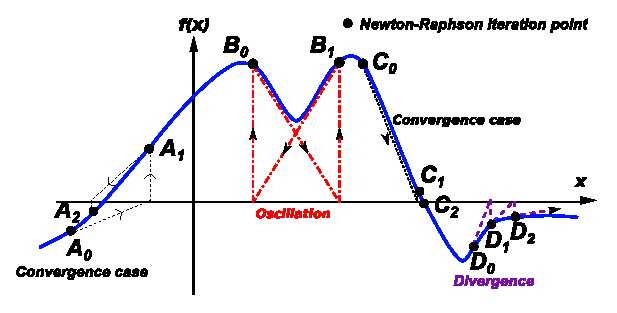
\includegraphics[width=8cm]{figs/divergencia.eps}
\caption{Casos de convergencia y divergencia en Newton-Raphson}
\label{NRG}
\end{figure}


Los problemas de convergencia (casos $B$ y $D$ ) en el m\'etodo de NR se vuelven m\'as dificiles conforme aumenta la complejidad de las ecuaciones debido a las altas no linealidades que se hacen presentes. De hecho, el m\'etodo de NR se empez\'o a usar desde el desarrollo el primer simulador de circuitos integrados SPICE \cite{homo_hspice} en 1975, en esa \'epoca los circuitos m\'as densos ten{\'i}an menos de 10,000 transistores por CI, lo que contrasta notoriamente con los  m\'as de 2 mil millones de transistores \cite{lmoore} que puede contener un CI actualmente; \'esto se traduce en un aumento abismal en el tama\~no y complejidad del problema a resolver por el m\'etodo de Newton. Aunado al aumento en el n\'umero de transistores tambi\'en se suma el aumento en complejidad de los modelos f{\'i}sicos que describen el comportamiento de los transistores actuales (por ser de dimensiones sub-microm\'etricas, lo que implica fen\'omenos f{\'i}sicos mucho m\'as complejos \cite{homo_BSIM}).  

El circuito ERDD de la figura \ref{2tunelx} est\'a compuesto  por arreglo en serie de: dos diodos t\'unel (K3, y K4), una resistencia (R2) y una fuente de voltaje (V1). 
\begin{figure}[hbtp]
\centerline{
\epsfxsize=70mm 
\epsffile{chap4/figs/erdd.eps}
}
\caption{Circuito con dos diodos tunel}
\label{2tunelx}  
\end{figure}



Los dos diodos t\'unel son id\'enticos presentando la siguiente funci\'on de rama:

\begin{displaymath}
i=I_p({V \over V_p})e^{1-{V \over V_p}}+I_0e^{{q \over {KT}} V}
\end{displaymath}
donde el valor para la fuente de voltaje $V_1$ es de $1V$ y para la resistencia  $R_2$ es de $20\Omega$. Adem\'as, ambos diodos t\'unel ($K_3$ y $K_4$) tiene el mismo
modelo con coeficientes:
$Ip=100 \times 10^{-3}$,
$V_p=50 \times 10^{-3} $, $I_0=1\times 10^{-9}$ y ${q \over {KT}} = 40$. 



Este circuito posee un total de 9 puntos de operaci\'on o soluciones, de las cuales los simuladores de circuitos integrados en el mejor de los casos pueden localizar solamente una soluci\'on. Se ejemplifica lo antes mencionado utilizando el simulador LTSpice IV \cite{LTSpice} para hacer un an\'alisis de CD del circuito de la figura 3. El punto de inicio elegido es  $v_1=v_2=v_3=v_4=2V$  para el m\'etodo NR. El resultado se muestra en la figura \ref{newtonfail} y es falta de convergencia en el m\'etodo de NR  ({\sf Direct Newton iteration failed to find .op point}). Este suceso es grave para el m\'etodo de NR ya que el circuito contiene s\'olo 4 transistores contra los circuitos comerciales que puede contener en el orden de millones de transistores (lo que se traduce en un radical aumento de complejidad de la ecuaci\'on de equilibrio). Una vez que el m\'etodo de NR falla el simulador ejecuta autom\'aticamente un m\'etodo num\'erico de respaldo llamado escalonamiento de conductancias \cite{homo_spectre,homo_hspice,homo_aplac}, el cual logra encontrar un punto de operaci\'on. De hecho, el escalonamiento
de conductacias es un tipo primitivo de homotop{\'i}a clasificado dentro de las homotop{\'i}as de tipo natural. 


\begin{figure*}[tbp]
\centering
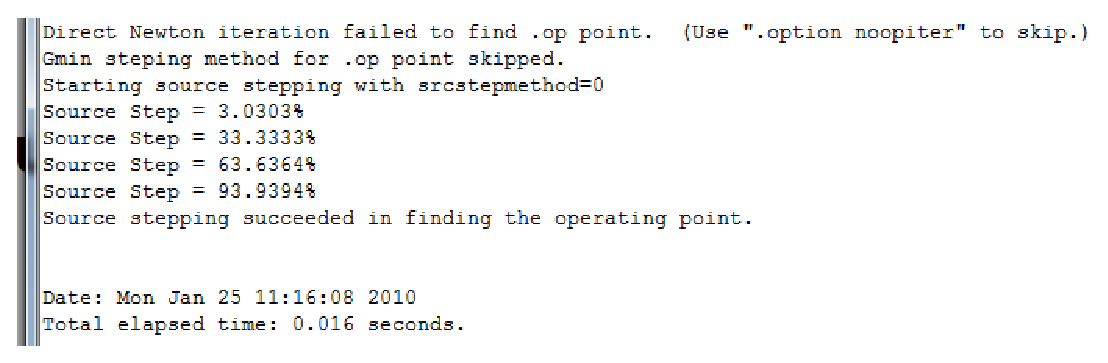
\includegraphics[width=15cm]{figs/newtonfail.eps}
\caption{Mensaje de error en el m\'etodo de Newton-Raphson en LTSPICE IV}
\label{newtonfail}
\end{figure*}

Los dise\~nadores de circuitos integrados tienen que lidiar cotidianamente con fallos de convergencia en el m\'etodo de NR y los m\'etodos de respaldo, por lo que como \'ultimo recurso se acude a modificar algunos par\'ametros del motor num\'erico del simulador esperando que se logre la convergencia. Esto situaci\'on aumenta los tiempos de dise\~no, haciendo m\'as costoso y lento el proceso completo del ciclo de dise\~no. Esta situaci\'on por si misma justifica el uso de m\'etodos alternativos al de Newton como la homotop{\'i}a para localizar el punto de operaci\'on. Sin embargo, existen m\'as razones para usar los m\'etodos de homotop{\'i}a, como la existencia de m\'ultiples puntos de operaci\'on. La raz\'on es que al contrario del m\'etodo de Newton, la homotop{\'i}a puede localizar m\'ultiples puntos de operaci\'on. Esto es de gran importancia ya que  podr{\'i}a darse la situaci\'on desastrosa de que el dise\~nador de por bueno un punto de operaci\'on en CD (encontrado por el m\'etodo de Newton) que no se presente f{\'i}sicamente en el circuito integrado ya fabricado. Esto se traduce en un mal funcionamiento del circuito con repercusiones costosas para la compa\~n{\'i}a.

Los m\'etodos de homotop{\'i}a \cite{BHLHOM,homo_ushida1,homo_green2,homo_DWolfMulti,homo_ArtificialP} han demostrado su utilidad para localizar m\'ultiples puntos de operaci\'on y para converger a las soluciones donde el m\'etodo de Newton no lo hace. Sin embargo, los m\'etodos de homotop{\'i}a son afectados por ciertos inconvenientes, entre los que podemos mencionar: el criterio de paro y tiempo de c\'omputo.  


\section{Homotop{\'i}a doblemente acotada}


Considerando la existencia de dos l{\'i}neas soluci\'on, una en
$\lambda=a$ y otra en $\lambda=b$ la formulaci\'on homot\'opica es la siguiente:


\begin{equation}
\pig{H}(\pig{f}(\pig{x}),\lambda ) =\pig{0}
\label{H2M}
\end{equation}
donde $\lambda$ es la variable homot\'opica y $\pig{H}^{-1}(\pig{0})$ la familia
de soluciones que conforma la trayectoria homot\'opica, de modo que:


\begin{itemize}
\item Para $\lambda=0.5(a+b)$ la soluci\'on de $H^{-1}(.)$ es conocida
o facil de obtener computacionalmente. Este punto se conoce como
punto de inicio de la homotop{\'i}a ($\lambda_i$).
\item Para $\lambda=a$, $\pig{H}(\pig{f}(\pig{x}),\pig{a} )=\pig{f}(\pig{x})$.
Esto significa que en $\lambda=a$ se encuentran todas las soluciones de $\pig{f}(\pig{x})$.
\item Para $\lambda=b$, $\pig{H}(\pig{f}(\pig{x}),\pig{b} )=\pig{f}(\pig{x})$.
Esto significa que en $\lambda=b$ se encuentran todas las soluciones de $\pig{f}(\pig{x})$.
\item La trayectoria de $\pig{H}^{-1}(\pig{0})$  es una funci\'on continua de $\lambda$ en el rango de $a \leq \lambda \leq b $. 
\end{itemize}

\section{Homotop\'{\i}a Polinomial Doblemente Acotada con 4 l{\'i}neas soluci\'on}

La {\bf Homotop\'{\i}a Polinomial Doblemente Acotada} con 4 l{\'i}neas soluci\'on (PDA4) esta definida por la siguiente ecuaci\'on:
\begin{equation}
{\small
\begin{array}{l}
\pig{H}(\pig{f}(\pig{x}),\lambda )=Q(x-x_i)(x-x_f) +C(\lambda-a/2)^2 \pig{f}(\pig{x})^2
\end{array}}
\label{homotopiaP}
\end{equation}
donde {\small $Q=\lambda(\lambda+a)(\lambda-a)(\lambda-2a)$}, $a$ es una constante que representa la separaci\'on entre las l\'{\i}neas soluci\'on, $x_i$ es el punto
de inicio, $x_f$ es el punto final y $C$ es una constante arbitraria.


En base a lo anterior, la homotopia se puede expresar de manera general como:
\begin{displaymath}
\pig{H}(\pig{f}(\pig{x}),\lambda ) = \left\{\begin{array}{rl}
f(x^*)=0 & \textrm{para $\lambda=0$ y $x=x^*$}\\
(x-x_i)(x-x_f)=0 & \textrm{para $\lambda=a/2$}\\
f(x^*)=0 & \textrm{para $\lambda=a$ y $x=x^*$}
\end{array}\right.
\end{displaymath}
donde $x^*$ es cualquier soluci\'on de $f(x)$ y $x_i$ y $x_f$ son los puntos inicial y final de la homotop{\'i}a respectivamente. 




Esta homotop\'{\i}a contiene 4 l\'{\i}neas soluci\'on ($\lambda=-a$, $\lambda=0$, $\lambda=a$ y $\lambda=2a$). Sin embargo, las dos l\'{\i}neas soluci\'on de los extremos son ramas
desconectadas que no se usan para fines de trazado. Elevar la funci\'on $f(x)$ al cuadrado tiene la finalidad de establecer un n\'umero par de soluciones reales (o puntos de operaci\'on) lo que
produce precisamente el acotamiento y cierre de la trayectoria homot\'opica dentro de la regi\'on intermedia.


\begin{figure*}[tbp]
{\tiny  
\centerline{
\psfrag{o}{$\lambda$}
\centering
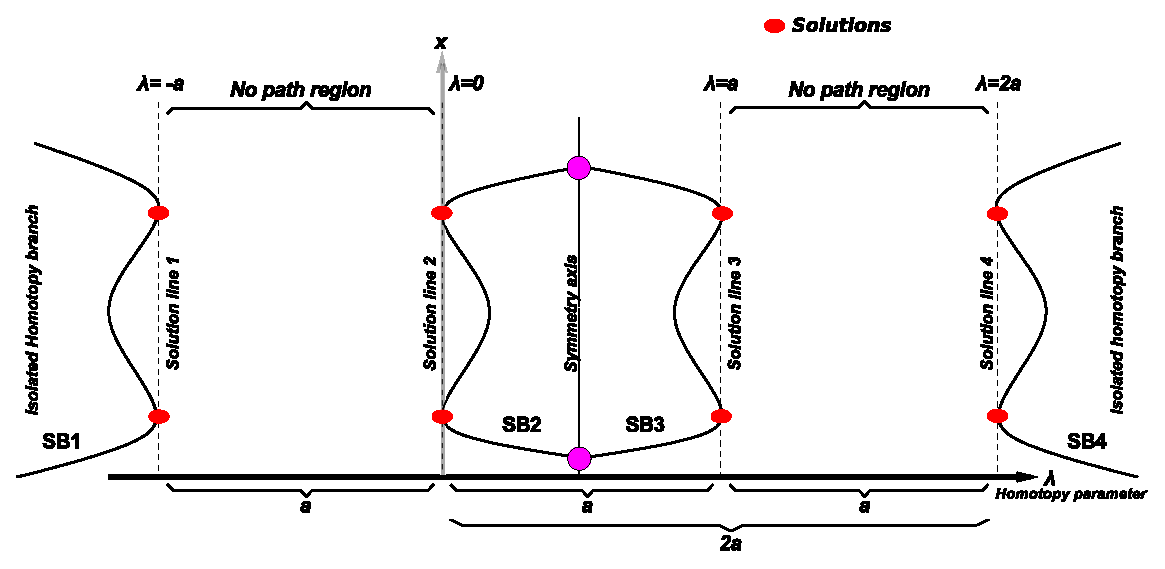
\includegraphics[width=14cm]{figs/doblelineapoli.eps}}}
\caption{Esquema general de una homotop\'ia polinomial con doble soluci\'on}
\label{doblehp}
\end{figure*}


En la figura  \ref{halftrack} se muestra como la trayectoria homot\'opica comienza en $A=(x_i,a/2)$ sobre
el eje de simetr\'{\i}a, encuentra las dos ra{\'i}ces (en la regi\'on $SB3$)  y finalmente t\'ermina cuando se detecta  un nuevo cruce por el eje de simetr\'{\i}a en $B=(x_f,a/2)$ lo que significa
que se completo el trazado de una rama sim\'etrica cumpli\'endose as\'{\i} el criterio de paro.


\begin{figure}[hbtp]
\psfrag{o}{$\lambda$}
\centering
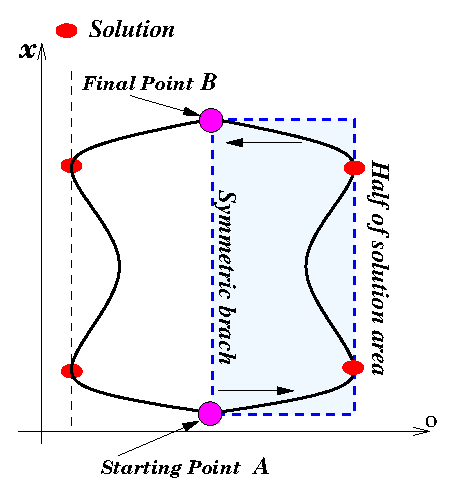
\includegraphics[width=2in]{figs/chap3/figs/dbh2.eps}
\caption{Stop Criteria}
\label{halftrack}
\end{figure}

Las propiedades de esta nueva homotop{\'i}a se presentan en las siguientes sub-secciones:

\subsection{Ramas sim\'etricas}

Para obtener las ramas de la trayectoria homot\'opica, en primera se reformula la ecuaci\'on \ref{homotopiaP} como sigue:

\begin{equation}
{%\tiny
\begin{array}{l}
\pig{H}(\pig{f}(\pig{x}),\lambda )=\lambda(\lambda+a)(\lambda-a)(\lambda-2a)+(\lambda-a/2)^2 J(x)=0
\end{array}}
\label{homotopiaP1}
\end{equation}
donde 
\begin{displaymath}
\begin{array}{l}
 J(x)= {Cf(x)^2 \over (x-x_i)(x-x_f)}
\end{array}
\end{displaymath}

Las ramas sim\'etricas mostradas en la figura \ref{doblehp}, se pueden obtener despejando $\lambda$ de la ecuaci\'on \ref{homotopiaP1}. 
El resultado
es 4 ramas sim\'etricas. Resultando que cada rama sim\'etrica {\it SB1, SB2, SB3} y {\it SB4} esta ligada una diferente l{\'i}nea soluci\'on $\lambda=[-a,0,a,2a]$ respectivamente.
Para fines de trazado de la trayectoria homot\'opica se ignorar\'a las ramas sim\'etricas desconectadas {\it SB1} y {\it SB4}, mismas que por
ser abiertas no permitir{\'i}an implementar algun criterio de paro. Dado que {\it SB2} y {\it SB3} estan conectadas y son sim\'etricas, s\'olo es necesario trazar una de ellas
para obtener la trayectoria completa y asi finalizar la simulaci\'on. Se elige {\it SB3} como la trayectoria a trazar, la cual toca tangencialmente a la l{\'i}nea soluci\'on $\lambda=a$.


\begin{table*}[tbp]
\center{ \large
\begin{tabular}{||c|c|c||}
\hline\hline
Rama sim\'etrica  & Formulaci\'on  & L{\'i}mite en $f(x^*)=0$   \\ \hline\hline \vspace{1mm}
{\it SB1} & $\lambda_1= {{a-\sqrt {5\,{a}^{2}+2\,\sqrt { \left( J \left( x \right) +4
\,{a}^{2} \right)  \left( J \left( x \right) +{a}^{2} \right) }+2\,J
 \left( x \right) }} \over {2}}$ & $\lambda=-a$ \\  \hline \vspace{1mm}
{\it SB2} & $\lambda_2= {{a-\sqrt {5\,{a}^{2}-2\,\sqrt { \left( J \left( x \right) +4
\,{a}^{2} \right)  \left( J \left( x \right) +{a}^{2} \right) }+2\,J
 \left( x \right) }} \over {2}}$  & $\lambda=0$ \\  \hline \vspace{1mm}
{\it SB3} & $\lambda_3= {{a+\sqrt {5\,{a}^{2}-2\,\sqrt { \left( J \left( x \right) +4
\,{a}^{2} \right)  \left( J \left( x \right) +{a}^{2} \right) }+2\,J
 \left( x \right) }} \over {2}}$ & $\lambda=a$ \\  \hline \vspace{1mm}
 {\it SB4} & $\lambda_4= {{a+\sqrt {5\,{a}^{2}+2\,\sqrt { \left( J \left( x \right) +4
\,{a}^{2} \right)  \left( J \left( x \right) +{a}^{2} \right) }+2\,J
 \left( x \right) }} \over {2}}$ & $\lambda=2a$ \\  \hline  \hline
\end{tabular}
}
\caption{Ramas sim\'etricas}
\label{ramasx}
\end{table*} 


\subsection{Eje de simetr\'ia}

El eje de simetr{\'i}a es una propiedad importante en las homotop{\'i}as doblemente acotadas. En el 
caso particular de la homotop{\'i}a polinomial doblemente acotada el eje de simetr{\'i}a es:

\begin{equation}
\lambda_{sym}= {a \over 2}
\label{sym}
\end{equation}
Este eje de simetr{\'i}a pertenece a la relaci\'on de simetr{\'i}a de las ramas $SB2$ y $SB3$.


Tal y como se muestra en la figura \ref{simetria} se debe cumplir la siguiente relaci\'on:
\begin{displaymath}
\lambda_3-\lambda_{sym}=\lambda_{sym} -\lambda_2
\end{displaymath}

Remplazando el valor de $\lambda_{sym}$ se obtiene que:
\begin{displaymath}
\lambda_3-0.5a=0.5a-\lambda_2
\end{displaymath}

Remplazando el valor de $\lambda_2$ y $\lambda_3$ por sus respectivas funciones se obtiene la siguiente relaci\'on:

\begin{displaymath}
\begin{array}{l}
0.5a+0.5\sqrt{G(\pig{x})}-0.5a= 0.5a-0.5a+0.5\sqrt{G(\pig{x})}
\end{array}
\end{displaymath}
donde {\small $G(\pig{x})=\sqrt {5\,{a}^{2}-2\,\sqrt { \left( J \left( x \right) +4 \,{a}^{2} \right)  \left( J \left( x \right) +{a}^{2} \right)}} $


Eliminando los terminos resulta:
\begin{displaymath}
\begin{array}{c}
0.5\sqrt{G(\pig{x})}=0.5\sqrt{G(\pig{x})} \\
0=0
\end{array}
\end{displaymath}
La comprobaci\'on de esta igualdad demuestra que la trayectoria de la homotop{\'i}a es sim\'etrica al rededor del eje de simetr{\'i}a.


{
\tiny
\begin{figure}[hbtp]
\psfrag{o}{\tiny $\lambda$}
\psfrag{o1}{\tiny $\lambda_3$}
\psfrag{o2}{\tiny $\lambda_2$}
\psfrag{o3}{\tiny $\lambda_3-\lambda_{sym}$}
\psfrag{o4}{\tiny $\lambda_{sym}-\lambda_2$}
\centering
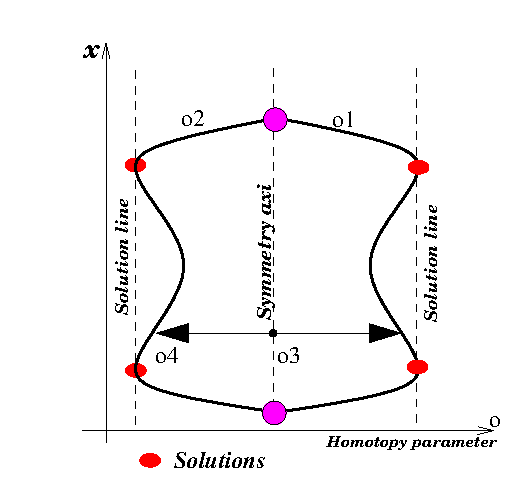
\includegraphics[width=9cm]{figs/simetria.eps}
\caption{Simetr\'{\i}a en la trayectoria homot\'opica}
\label{simetria}
\end{figure}
}



\subsection{Punto de inicio y punto final}

El punto donde inicia la trayectoria homot\'opica se encuentra justo en el eje de simetr\'{\i}a 
por lo que $\lambda_i=a/2$. Por lo tanto, reemplazando $\lambda_i$ en la ecuaci\'on \ref{homotopiaP} se cancela el termino que contiene la ecuaci\'on de equilibrio $f(x)$, resultando:
\begin{displaymath}
\begin{array}{r}
\pig{H}(\pig{f}(\pig{x}),\lambda_i )=(x-x_i)(x-x_f)=0  \\
\end{array}
\end{displaymath}
Por lo tanto, el punto de inicio $x_i$  y final $x_f$ son elegidos arbitrariamente.


Despejando $\lambda$ de la ecuaci\'on \ref{homotopiaP} se obtiene que para la rama SB3:
{
%\tiny
\begin{displaymath}
\lambda_3= {\frac {Fa+\sqrt {5\,{F}^{2}{a}^{2}-2\,F\sqrt { 4\,{F}^{2}{a}^
{4}+5\,F \left( f \left( x \right)  \right) ^{2}{a}^{2}+ \left( f
 \left( x \right)  \right) ^{4}}+2\,F \left( f \left( x \right) 
 \right) ^{2}}}{2F}}
\end{displaymath}
}
donde $F=(x-x_i)(x-x_f)$. Ahora se calculan los siguientes l{\'i}mites:

\begin{equation}
 \displaystyle\lim_{x \to{x_i}}{\lambda_3}=0.5a 
 \label{demos1}
\end{equation}

\begin{equation}
  \displaystyle\lim_{x \to{x_f}}{\lambda_3}=0.5a
 \label{demos1}
\end{equation}

Por lo tanto, cuando $x$ tiende al valor del punto de inicio $x_i$ o punto final $x_f$,  el par\'ametro homot\'opico $\lambda$ tiende al eje de simetr{\'i}a en $\lambda=0.5a$.




\subsection{Interpretaci\'on Circuital}


La interpretaci\'on circuital de la homotop{\'i}a doblemente acotada se puede derivar
despejando $f(x)$ de la expresi\'on de la homotop\'ia de la ecuaci\'on \ref{homotopiaP}. De dicha ecuaci\'on se puede deducir que existen fuentes no lineales de corriente ($K_1$, · · · ,$K_n$) conectadas a cada nodo del circuito, donde $n$ es el n\'umero de nodos y $l$ el n\'umero de fuentes de voltaje constantes ($E$). 

\begin{equation}
I_{K_i}={\lambda(\lambda+a)(\lambda-a)(\lambda-2a)(V_{xk}-V_{{xk}_i})(V_x-V_{xk_f}) \over (\lambda-a/2)^2}
\label{Ikn}
\end{equation}
donde $k=[1,n]$,  $V_{xk}$ son los voltajes nodales del circuito, $V_{{xk}_i}$ y $V_{{xk}_f}$ son constantes relacionadas con el punto de inicio y fin de cada variable $V_{xk}$ de la homotop{\'i}a.
Finalmente, la
interpretaci\'on circuital de la homotop{\'i}a en el eje de simetr{\'i}a se puede observar en la
figura \ref{circ1}.


\begin{figure*}[tbp]
\centerline{
\epsfxsize=140mm
\epsffile{figs/circ.eps}}
\caption{Interpretaci\'on circuital de la Homotopia L Doblemente Acotada}
\label{circ1}
\end{figure*}


\subsection{M\'ultiples Variables}


Cuando la homotop\'{\i}a es aplicada a un sistema de ecuaciones no lineales con m\'ultiples variables, la generalizaci\'on est\'a dada por:

\begin{displaymath}
\begin{array}{c}
H_1(f_1(x),\lambda)=Q(x_1-x_i)(x_1-x_f)+C(\lambda-a/2)^2f_1(x)^2 \vspace{5mm} \\
H_2(f_2(x),\lambda)=Q(x_2-x_i)(x_2-x_f)+C(\lambda-a/2)^2f_2(x)^2 \vspace{5mm} \\
H_3(f_3(x),\lambda)=Q(x_3-x_i)(x_3-x_f)+C(\lambda-a/2)^2f_3(x)^2 \\
\vdots  \hspace{30mm} \vdots  \hspace{30mm} \vdots \\
H_n(f_n(x),\lambda)=Q(x_n-x_i)(x_n-x_f)+C(\lambda-a/2)^2f_n(x)^2 \\
\end{array}
\end{displaymath}
donde $n$ es el n\'umero de ecuaciones de la ecuaci\'on de equilibrio $\pig{f}(\pig{x})$, $f_i$ representa a cada una de las ecuaciones nodales o ecuaciones extra de elementos
no-NA compatibles \cite{mnaxx}, $C$ es una constante arbitraria y $Q=\lambda(\lambda+a)(\lambda-a)(\lambda-2a)$.


En la figura \ref{poligono} se presenta un poligono el cual muestra de manera descriptiva el comportamiento de las posibles trayectorias homot\'opicas partiendo desde diferentes
puntos de inicio, resultantes de las combinaciones del punto de inicio y fin de cada $x$. Por lo tanto, cada vertice representa es un posible punto de inicio o fin de la trayectoria homot\'opica.
A continuaci\'on
se describen algunos casos posibles. En n\'umero total de vertices del poligono es $n^2$.



\begin{itemize} 
\item En el caso del punto $p_1$ la trayectoria homot\'opica termina en $p_5$, cruzando por 3 puntos de operaci\'on ($S_1$, $S_2$, y $S_3$).
\item En el caso del punto $p_2$ la trayectoria homot\'opica termina en $p_4$, cruzando por 2 puntos de operaci\'on ($S_2$ y $S_3$), los cuales 
son comunes a la trayectoria descrita por $p_1-p_5$.
\item En el caso del punto $p_3$ la trayectoria homot\'opica termina en $p_{(n^2)}$, cruzando por 3 punto de operaci\'on ($S_1$, $S_2$, y $S_3$), los cuales 
son comunes a la trayectoria descrita por $p_1-p_5$.
\end{itemize}

\begin{figure*}[tbp]
\psfrag{p1}{\tiny $p_1=({x1}_i,{x2}_i,{x3}_i,...,{xn}_i,\lambda=0.5a)$}
\psfrag{p2}{\tiny $p_2=({x1}_i,{x2}_f,{x3}_i,...,{xn}_i,\lambda=0.5a)$}
\psfrag{p3}{\tiny $p_3=({x1}_i,{x2}_i,{x3}_f,...,{xn}_f,\lambda=0.5a)$}
\psfrag{p4}{\tiny $p_4=({x1}_i,{x2}_f,{x3}_f,...,{xn}_i,\lambda=0.5a)$}
\psfrag{p5}{\tiny $p_5=({x1}_f,{x2}_i,{x3}_i,...,{xn}_i,\lambda=0.5a)$}
\psfrag{p6}{\tiny $p_{(n^2)}=({x1}_f,{x2}_f,{x3}_f,...,{xn}_f,\lambda=0.5a)$}
\psfrag{x1}{\tiny $(S_1,\lambda=a)$}
\psfrag{x2}{\tiny $(S_2,\lambda=a)$}
\psfrag{x3}{\tiny $(S_3,\lambda=a)$}
\centering
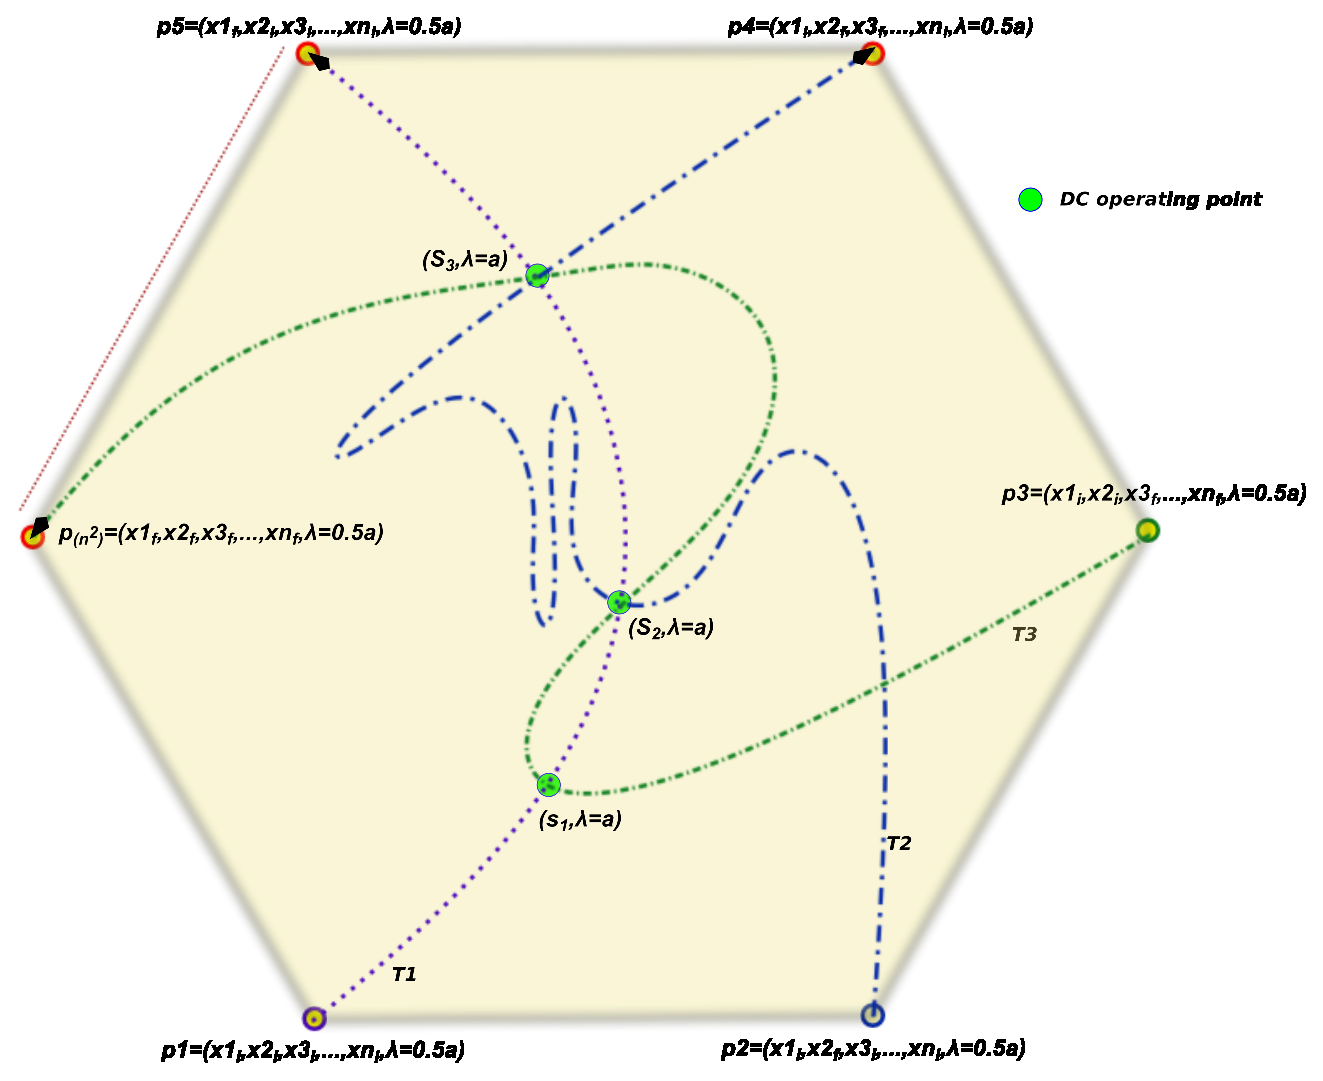
\includegraphics[width=12cm]{figs/poligono.eps}
\caption{Vertices de puntos de inicio y fin de la trayectoria homot\'opica}
\label{poligono}
\end{figure*}

\subsection{Radio de Curvatura}

El radio de curvatura de la trayectoria homot\'opica se utilizar\'a como herramienta para analizar {\it cualitativamente} 
el comportamiento
de las trayectorias en los puntos estrat\'egicos como las soluciones y los puntos de retorno (ver figura \ref{radio1}).
El radio de curvatura de una curva en un punto es el radio del c\'{\i}rculo con la curvatura equivalente en ese punto de la curva.
La ecuaci\'on del radio de curvatura es:

\begin{displaymath}
\rho=  \Bigg |{{(1 + (y')^2)^{3/2}} \over {y''}} \Bigg |
\end{displaymath}
donde $y$ es una funci\'on $y(x)$, $y'$ es la primer derivada de $y(x)$ respecto de $x$ y
$y''$ es la segunda derivada de $y(x)$ respecto de $x$. En t\'erminos de la trayectoria homot\'opica
la primer derivada $y'$ es igual a ${ {d \lambda} \over {dx}}$ y la segunda derivada $y''$ es igual a ${ {d^2 \lambda} \over {dx^2}}$.



\begin{figure}[hbtp]
\psfrag{l}{$\lambda$}
\psfrag{z}{$\rho_s$}
\psfrag{v}{$\rho_r$}
\centering
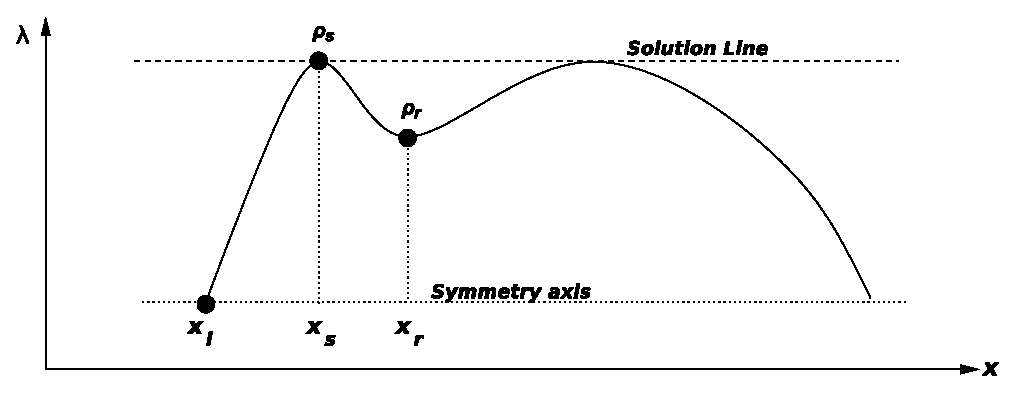
\includegraphics[width=8cm]{figs/chap3/figs/radiob.eps}
\caption{Punto de soluci\'on $\rho_s$ y punto de retorno $\rho_r$}
\label{radio1}
\end{figure}


La pendiente de la trayectoria homot\'opica en los puntos de las soluciones y retornos tiene pendiente cero ($y'={ {d \lambda} \over {dx}} =0$),
propiedad que se puede utilizar para simplificar la expresi\'on del radio de curvatura en esos puntos, como:


\begin{displaymath}
\rho= \Bigg | {1 \over {{ {d^2 \lambda} \over {dx^2}}}} \Bigg |
\end{displaymath}



Ahora, se procede a derivar  dos veces $\lambda_3$ de la ecuaci\'on SB3 de la tabla \ref{ramasx}, con respecto a $x$, considerando $a$, y $C$ como
constantes. Despu\'es de derivar se reemplaza  $f(x)$ por cero ya que es
el punto de la soluci\'on, resultando:
\begin{displaymath}
\rho_{s}=\left[4\,{\frac {a \left( x-x_i \right)  \left( x+x_f \right) }{  C
   \left( {\frac {d}{dx}}f \left( x \right) \right)^{2}}}\right]_{x=x_s}
\end{displaymath}
donde $x_s$ es el valor de la soluci\'on y  $a$ representa a la separaci\'on entre las l\'{\i}neas soluci\'on.


La ecuaci\'on $\rho_{s}$ permite concluir que la distancia $a$ entre las l\'{\i}neas soluci\'on
afecta lo aguzado de la trayectoria homot\'opica en las soluciones, de tal modo
que la curva se aguza m\'as conforme las l\'{\i}neas soluci\'on se acercan (entre ellas) y se aplana
conforme las l\'{\i}neas soluci\'on se alejan. Adem\'as, la constante $C$ afecta
la curva, aplanandose \'esta en la soluci\'on cuando $C$ se incrementa y por
el contrario, aguzandose conforme $C$ decrece.


El punto donde la trayectoria retorna en la busqueda de soluciones se denomina
punto de retorno $\rho_r$. El estudio del radio de curvatura en el punto de retorno $\rho_r$
se complementa con el estudio del radio de curvatura en las soluciones $\rho_s$ con la finalidad
de comprender con m\'as profundidad el comportamiento cualitativo de la trayectoria homot\'opica.
En el punto de retorno la derivada de la $\lambda$ con respecto
de $x$ es igual a cero. Adem\'as,  el punto de retorno coincide espacialmente con los puntos cr\'{\i}ticos de la funci\'on
$f(x)$, por lo que la derivada de $f(x)$ con respecto de $x$ es igual a cero. 

Con la finalidad de simplificar la ecuaci\'on del radio de curvatura se asume que: 
\begin{displaymath}
\begin{array}{l}
 j(x)= {f(x)^2 \over (x-x_i)(x-x_f)}
\end{array}
\end{displaymath}
Por lo tanto, la ecuaci\'on del radio de curvatura queda como:
{
%\tiny
\begin{displaymath}
\rho_{r}=\left[{4\,\sqrt {5\,{a}^{2}- 2\,\sqrt {4\,{a}^{4}+ 5\,Cj \left( x
 \right) {a}^{2}+{C}^{2} \left( j \left( x \right)  \right) ^{2}}+ 2
\,Cj \left( x \right) } \over \left( -{\frac {5\,C \left( {\frac {d^{2}}{d{x
}^{2}}}j \left( x \right)  \right) {a}^{2}+2\,{C}^{2}j \left( x
 \right) {\frac {d^{2}}{d{x}^{2}}}j \left( x \right) }{\sqrt {4\,{a}^{
4}+5\,Cj \left( x \right) {a}^{2}+{C}^{2} \left( j \left( x \right) 
 \right) ^{2}}}}+2\,C{\frac {d^{2}}{d{x}^{2}}}j \left( x \right) 
 \right)} \right]_{x=x_r}
\end{displaymath}
}
donde $x_r$ es el valor de $x$ en el punto de retorno.




Para evaluar cualitativamente el comportamiento del radio de curvatura es necesario realizar los siguientes l{\'i}mites simb\'olicos:

\begin{equation}
 \displaystyle\lim_{f(x) \to{+}\infty}{|\rho_{r}|}=\infty
 \label{rcurv1}
\end{equation}

\begin{equation}
 \displaystyle\lim_{f(x) \to{+}0}{|\rho_{r}|}= \left[8\,{\frac {a}{C{\frac {d^{2}}{d{x}^{2}}}f \left( x \right) }} \right]_{x=x_r} 
  \label{rcurv2}
\end{equation}

El l\'{i}mite de la ecuaci\'on \ref{rcurv1} indica que cuando $f(x)$ tiende a valores grandes, el radio de curvatura crece, dejando la curva aplanada.
El caso cuando $f(x)$ tiene valores grandes (evaluada en el punto de retorno $x_r$) es bastante com\'un en las ecuaciones nodales de los circuitos. Por lo tanto,
la trayectoria homot\'opica tendera a quedarse en la cercania de la l{\'i}nea soluci\'on $\lambda=a$.
Suponga que se resuelve la trayectoria de una homotopia polinomial doblemente acotada con $a=1$. 
En la figura \ref{xxx1}(a) se muestra la rama sim\'etrica derecha correspondiente a $\lambda=1$. En dicha figura no se puede
apreciar facilmente la diferencia entre los puntos de retorno y las soluciones mismas.
Un acercamiento a la l{\'i}nea soluci\'on $\lambda=1$ (ver Figura \ref{xxx1}(b))
permite observar m\'as claramente las soluciones y sus puntos de retorno. Este fen\'omeno se 
corrobor\'o mediante simulaciones de diversos circuitos y ecuaciones no lineales. 
El l\'{i}mite de la ecuaci\'on \ref{rcurv2} indica que cuando $f(x)$ tiende a valores peque\~nos, el radio de curvatura es proporcional al valor de la l{\'i}nea soluci\'on $a$
e inversamente proporcional a la constante $C$.





\begin{figure}[hbtp]
\centering
\includegraphics[width=2.5in]{figs/curvatura.eps}
\caption{a) Trayectoria homot\'opica t{\'i}pica b) Acercamiento a la regi\'on de las soluciones}
\label{xxx1}
\end{figure}

\section{Casos de estudio}

La homotop\'{\i}a doblemente acotada se ha desarrollado con la finalidad
de simular circuitos no lineales con m\'ultiples soluciones.
En esta secci\'on se muestra la simulaci\'on homot\'opica de diferentes tipos de circuitos con la finalidad de exponer
el nuevo m\'etodo propuesto a una variedad de funciones no lineales.


\subsection{Caso matem\'atico}

Con la finalidad de ilustrar el uso de la homotop\'{\i}a para un ejemplo
bi-dimensional, la homotop\'{\i}a es aplicada
al siguiente sistema de NAEs:
\begin{displaymath}
\begin{array}{c}
f_1(x_1,x_2)=(x_2-1)(x_2-4)(x_2-6)+x_1=0\\
f_2(x_1,x_2)=(x_1-3)(x_1-6)(x_1-9)+x_2=0
\end{array}
\end{displaymath}
La soluci\'on gr\'afica del sistema se muestra en la figura \ref{9sol}.

\begin{figure}[hbtp]
\centerline{
\epsfxsize=80mm
\epsffile{chap3/figs/doblelimit_mul.eps}}
\caption{Sistema con cinco soluciones}
\label{9sol}
\end{figure}


La formulaci\'on homot\'opica propuesta es:
\begin{displaymath}
\begin{array}{c}
H_1(f_1,\lambda)=\lambda(\lambda+1)(\lambda-1)(\lambda-2)(x_1-13)(x_1+13)+(\lambda-0.5)^2 f_1^2=0\\
H_2(f_2,\lambda)=\lambda(\lambda+1)(\lambda-1)(\lambda-2)(x_2-13)(x_2+13)+(\lambda-0.5)^2 f_2^2=0\\
\end{array}
\end{displaymath}
donde la l{\'i}nea soluci\'on se encuentra en $\lambda=0$ y $\lambda=1$. Para fines pr\'acticos s\'olo se traza la rama sim\'etrica
de la trayectoria homot\'opica que esta ligada a la l{\'i}nea soluci\'on $\lambda=1$.

Se elije como punto de inicio $A=[x_1=-13,x_2=-13]$ y se inicia el trazado de la trayectoria, resultando una convergencia global a todas
las soluciones del sistema ($S_1,S_2,S_3,S_4$ y $S_5$) (Ver figura \ref{homotex}). El punto final resulta ser $B=[x_1=13, x_2=13]$ y la trayectoria homot\'opica  para
cada variable ($x_1-\lambda$ y $x_2-\lambda$) se muestra en las figuras \ref{xxx1} y \ref{xxx2}.

\begin{figure}[hbtp]
\psfrag{ll}{$\lambda=1.5$}
\psfrag{l}{$\lambda$}
\psfrag{l1}{$\lambda=2$}
\psfrag{x}{$x_1$}
\psfrag{y}{$x_2$}
\centerline{
\epsfxsize=80mm
\epsffile{ejem4lim/POLINOM4LIMA.eps}}
\caption{Trayectoria homot\'opica para ejemplo de 2 variables}
\label{homotex}
\end{figure}

\begin{figure}[hbtp]
\psfrag{ll}{$\lambda=1.5$}
\psfrag{l}{$\lambda$}
\psfrag{l1}{$\lambda=2$}
\psfrag{x}{$x_1$}
\psfrag{y}{$x_2$}
\centerline{
\epsfxsize=80mm
\epsffile{ejem4lim/POLINOM4LIMAx1.eps}}
\caption{Trayectoria homot\'opica $x_1-\lambda$}
\label{xxx1}
\end{figure}

\begin{figure}[hbtp]
\psfrag{ll}{$\lambda=1.5$}
\psfrag{l}{$\lambda$}
\psfrag{l1}{$\lambda=2$}
\psfrag{x}{$x_1$}
\psfrag{y}{$x_2$}
\centerline{
\epsfxsize=80mm
\epsffile{ejem4lim/POLINOM4LIMAx2.eps}}
\caption{Trayectoria homot\'opica $x_2-\lambda$}
\label{xxx2}
\end{figure}



\subsection{Circuito con dos diodos t\'unel}


Los diodos t\'unel tienen una comportamiento no lineal, el
cual se describe en forma general en la figura \ref{tunelmod}.
Como se puede observar en esta figura, el diodo t\'unel
contiene 3 cambios de signo en la pendiente lo que en combinaci\'on con una
recta de carga puede producir hasta 3 soluciones por diodo t\'unel
presente en el circuito. El modelo de diodo t\'unel elegido para este
ejemplo esta en funci\'on de t\'erminos exponenciales
\cite{homo_sze},\cite{homo_shur} y se puede expresar como:

\begin{displaymath}
i=I_p({V \over V_p})e^{1-{V \over V_p}}+I_0e^{{q \over {KT}} V}
\end{displaymath}

%\newpage



Los t\'erminos exponenciales pueden producir sobreflujos num\'ericos por lo que
este circuito
presenta un reto a la presente homotop{\'i}a doblemente acotada.
Por lo tanto, en este ejemplo se presenta un circuito (ERDD)
con 2 diodos t\'unel, una fuente de voltaje y
una resistencia en serie en la figura \ref{2tunel}. El valor para la fuente de voltaje $V_1$ es de $1V$ y para la resistencia  $R_2$ es de $20\Omega$. Adem\'as, ambos diodos t\'unel ($K_3$ y $K_4$) tiene el mismo
modelo con coeficientes:
$Ip=100 \times 10^{-3}$,
$V_p=50 \times 10^{-3} $, $I_0=1\times 10^{-9}$ y ${q \over {KT}} = 40$. La ecuaci\'on de equilibrio se formula a partir del an\'alisis
nodal modificado. Adem\'as, el sistema se reduce a 3 ecuaciones
eliminando el voltaje nodal $v_1$ por ser constante e igual
a la fuente de voltaje. Por lo tanto, las variables del sistema resultante son:
$I_E$, $v_2$ y $v_3$. Las ecuaciones quedan expresadas como:

\begin{displaymath}
\begin{array}{l}
f_1=  {1 \over 20}-{v_2 \over 20}+I_E =0\\ \\
f_2=  -{1 \over 20}+{v_2 \over 20}+2(v_2-v_3)e^{(1-20v_2+20v_3)} \\+1\times 10^{-9}e^{(40v_2-40v_3)} =0 \\\\
f_3=  2(v_2-v_3)e^{(1-20v_2+20v_3)}+1\times 10^{-9}e^{(40v_2-40v_3)} \\ 
-2v_3e^{(1-20v_3)}-1\times 10^{-9} e^{(40v_3)} =0
\end{array}
\end{displaymath}

\begin{figure}[hbtp]
\centerline{
\epsfxsize=55mm
\epsffile{chap4/figs/tunnelmod.eps}
}
\caption{Modelo del diodo t\'unel}
\label{tunelmod}
\end{figure}

\begin{figure}[hbtp]
\centerline{
\epsfxsize=70mm 
\epsffile{chap4/figs/erdd.eps}
}
\caption{Circuito con dos diodos tunel}
\label{2tunel}  
\end{figure}



%La gr\'afica
%del modelo para tales valores se muestra en la figura \ref{tunelmodn}.






Ahora, se aplica la  HDA para resolver el circuito,
La formulaci\'on homot\'opica se expresa como sigue:

\begin{displaymath}
\begin{array}{c}
H_1(f_1,\lambda)=\lambda(\lambda+1)(\lambda-1)(\lambda-2)(I_E-1)(I_E+1)+(\lambda-0.5)^2 f_1^2=0\\
H_2(f_2,\lambda)=\lambda(\lambda+1)(\lambda-1)(\lambda-2)(v_2-1)(v_2+1)+(\lambda-0.5)^2 f_2^2=0\\
H_3(f_3,\lambda)=\lambda(\lambda+1)(\lambda-1)(\lambda-2)(v_3-1)(v_3+1)+(\lambda-0.5)^2 f_3^2=0\\
\end{array}
\end{displaymath}
donde las l\'{\i}neas acotantes tiene un valor de $a=0$ y $b=1$, y el punto
de inicio de la trayectoria homot\'opica es seleccionado en $A=[I_E=-1,v_2=-1,v_3=-1]$.


Como resultado del trazado de la trayectoria homot\'opica,
se localizaron todas los puntos de operaci\'on  del circuito, en total  9. 
Adem\'as, el punto final de la trayectoria fue en $B=[I_E=1,v_2=1,v_3=1$.
En la figura \ref{2tunelg}(b) se muestra una ampliaci\'on de la regi\'on de la soluciones,
aqu\'{\i} se puede observar como la trayectoria cruza por las 9 soluciones, presentando 3 sub-regiones  ($F1$, $F2$ y $F3$)
de ra\'{\i}ces cercanas.
Con la finalidad de observar a detalle el comportamiento de la trayectoria
se realiza un ampliaci\'on para cada una de las regiones $F1$, $F2$ y $F3$ (ver
figuras \ref{2tunelg}(c), \ref{2tunelg}(d) y \ref{2tunelg}(e)).
En estas figuras se muestran las 9 soluciones ($S_1, S_2, S_3, S_4, S_5, S_6, S_7, S_8$ y $S_9$) sobre la trayectoria
homot\'opica. 

 
\begin{figure}[hbtp]
\centerline{
\epsfxsize=30mm
\epsffile{ejem4lim/TUNEL1.eps}\newline \\
\epsfxsize=30mm
\epsffile{ejem4lim/TUNEL2.eps} 
\epsfxsize=30mm
\epsffile{ejem4lim/TUNEL3.eps}\newline \\
\epsfxsize=30mm
\epsffile{ejem4lim/TUNEL4.eps} 
\epsfxsize=30mm
\epsffile{ejem4lim/TUNEL5.eps}
}
\caption{Trayectoria homot\'opica para el circuito con diodos tunel}
\label{2tunelg}
\end{figure}



\subsection{Circuito con transistores bipolares y un diodo}

Un circuito con transistores bipolares y un diodo circuito fue reportado en \cite{homo_tadeusiewicz} y  \cite{homo_yamamurawise}  y resuelto
mediante m\'etodos piecewise.
Posteriormente, en \cite{homo_yamamura}, el circuito fue resuelto mediante la homotop\'{\i}a de punto fijo modificada.
El circuito posee 3 puntos de operaci\'on. El modelo de Ebers-Moll es utilizado para todos los transistores.
La ecuaci\'on del modelo
esta dada como:

\begin{displaymath}
\left[ \begin{array}{c}
i_{D_E} \\
i_{D_C}
\end{array}\right] =
\left[ \begin{array}{cc} 1  & \alpha_R \\
\alpha_F & 1 \\
\end{array}\right] \left[ \begin{array}{c}
10^{-9}(e^{(40v_{be})} - 1) \\
10^{-9}(e^{(40v_{bc})} - 1)
\end{array}\right]
\end{displaymath}
Y la representaci\'on circuital del modelo se presenta en la figura \ref{FEbersMoll}.

El modelo del diodo es:

\begin{displaymath}
i_d=10^{-9}(e^{40u} - 1)
\end{displaymath}




\begin{figure*}[tbp]
\centerline{
\epsfxsize=110mm
\epsffile{chap4/figs/diotran.eps}
}
\caption{Circuito con transistores bipolares y diodo}
\label{yamamuracircuito}
\end{figure*}

%\end{minipage}


\begin{figure}[hbtp]
\psfrag{f}{$\alpha_F$}
\psfrag{r}{$\alpha_R$}
\centerline{
\epsfxsize=36mm
\epsffile{chap4/figs/ebersmoll.eps}}
\caption{Modelo Ebers-Moll del transistor bipolar}
\label{FEbersMoll}
\end{figure}


Los valores de los componentes del circuito se encuentran en la tabla \ref{yamamuracircuitovalores}.
Primero se formula la ecuaci\'on de equilibrio usando en el an\'alisis nodal modificado
quedando un sistema con 14 ecuaciones y 14 variables. 
El circuito se muestra en la figura \ref{yamamuracircuito} y su ecuaci\'on de equilibrio es la \ref{eqsd} (utilizando el m\'etodo de an\'alisis MNA).



\begin{table}[hbtp]
\center{
{\scriptsize
\begin{tabular}{||c|c||}
\hline\hline
Componente  & Valor  \\ \hline\hline
$R_1$ & $4K\Omega$   \\ \hline
$R_2$ & $0.1K\Omega$   \\ \hline
$R_3$ & $8K\Omega$   \\ \hline
$R_4$ & $8K\Omega$   \\ \hline
$R_5$ & $4K\Omega$   \\ \hline
$R_6$ & $0.1K\Omega$   \\ \hline
$R_7$ & $30K\Omega$   \\ \hline
$R_8$ & $1K\Omega$   \\ \hline
$R_9$ & $0.1K\Omega$   \\ \hline
$R_{10}$ & $10K\Omega$   \\ \hline
$R_{11}$ & $4K\Omega$   \\ \hline
$R_{12}$ & $10K\Omega$   \\ \hline
$R_{13}$ & $1K\Omega$   \\ \hline
$V_{cc}$ & $12V$   \\ \hline  \hline
\end{tabular}
}
}
\caption{Componentes del circuito}
\label{yamamuracircuitovalores}
\end{table}



{\tiny
\begin{equation}
\begin{array}{|r||r|} 
f_1 & {\frac {37}{20000}}\,{\it v_1}-{\frac {1}{4000}}\,{\it v_2}-{\frac {1}{
 4000}}\,{\it v_6}-{\frac {1}{1000}}\,{\it v_9}-{\frac {1}{4000}}\,{\it 
v_{12}}-{\frac {1}{10000}}\,{\it v_{13}}+{\it IE}=0 \\  
f_2 & -{\frac {1}{4000}}\,{\it v_1}+{\frac {3}{8000}}\,{\it v_2}-{\frac {1}{
8000}}\,{\it v_5}+ 0.00000000990\,{{\rm e}^{40\,{\it v_4}-40\,{\it v_3}}}
+ 0.00000000010- 0.000000010\,{{\rm e}^{40\,{\it v_4}-40\,{\it v_2}}}=0  \\  
f_3 & {\frac {1}{100}}\,{\it v_3}- 0.000000010\,{{\rm e}^{40\,{\it v_4}-40\,{
\it v_3}}}+ 0.00000000990+ 0.00000000010\,{{\rm e}^{40\,{\it v_4}-40\,{
\it v_2}}}=0 \\
f_4 & {\frac {1}{8000}}\,{\it v_4}-{\frac {1}{8000}}\,{\it v_6}+ 0.00000000010
\,{{\rm e}^{40\,{\it v_4}-40\,{\it v_3}}}- 0.00000001000+ 0.00000000990
\,{{\rm e}^{40\,{\it v_4}-40\,{\it v_2}}}=0 \\
f_5 & -{\frac {1}{8000}}\,{\it v_2}+{\frac {1}{8000}}\,{\it v_5}+
 0.00000000010\,{{\rm e}^{40\,{\it v_5}-40\,{\it v_7}}}- 0.00000001000+
 0.00000000990\,{{\rm e}^{40\,{\it v_5}-40\,{\it v_6}}}=0 \\
f_6 & -{\frac {1}{4000}}\,{\it v_1}-{\frac {1}{8000}}\,{\it v_4}+{\frac {3}{
8000}}\,{\it v_6}+ 0.00000000990\,{{\rm e}^{40\,{\it v_5}-40\,{\it v_7}}}
+ 0.00000001010- 0.000000010\,{{\rm e}^{40\,{\it v_5}-40\,{\it v_6}}}-
 0.000000010\,{{\rm e}^{40\,{\it v_8}-40\,{\it v_6}}}=0 \\
f_7 & {\frac {1}{100}}\,{\it v_7}- 0.000000010\,{{\rm e}^{40\,{\it v_5}-40\,{
\it v_7}}}+ 0.00000000990+ 0.00000000010\,{{\rm e}^{40\,{\it v_5}-40\,{
\it v_6}}}=0 \\
f_8 & {\frac {1}{30000}}\,{\it v_8}-{\frac {1}{30000}}\,{\it v_9}+ 0.000000010
\,{{\rm e}^{40\,{\it v_8}-40\,{\it v_6}}}- 0.000000010=0 \\
f_9 & -{\frac {1}{1000}}\,{\it v_1}-{\frac {1}{30000}}\,{\it v_8}+{\frac {31}{
30000}}\,{\it v_9}+ 0.00000000990\,{{\rm e}^{40\,{\it v_{11}}-40\,{\it v_{10}
}}}+ 0.00000000010- 0.000000010\,{{\rm e}^{40\,{\it v_{11}}-40\,{\it v_9}}
}=0 \\
f_{10} & {\frac {1}{100}}\,{\it v_{10}}- 0.000000010\,{{\rm e}^{40\,{\it v_{11}}-40\,
{\it v_{10}}}}+ 0.00000000990+ 0.00000000010\,{{\rm e}^{40\,{\it v_{11}}-40
\,{\it v_9}}}=0 \\
f_{11} & {\frac {1}{10000}}\,{\it v_{11}}-{\frac {1}{10000}}\,{\it v_{12}}+
 0.00000000010\,{{\rm e}^{40\,{\it v_{11}}-40\,{\it v_{10}}}}- 0.00000001000
+ 0.00000000990\,{{\rm e}^{40\,{\it v_{11}}-40\,{\it v_9}}}=0 \\
f_{12} & -{\frac {1}{4000}}\,{\it v_1}-{\frac {1}{10000}}\,{\it v_{11}}+{\frac {7}{
20000}}\,{\it v_{12}}+ 0.00000000990\,{{\rm e}^{40\,{\it v_{13}}}}+
 0.00000000010- 0.000000010\,{{\rm e}^{40\,{\it v_{13}}-40\,{\it v_{12}}}}=0 \\
f_{13} & -{\frac {1}{10000}}\,{\it v_1}+{\frac {11}{10000}}\,{\it v_{13}}+
 0.00000000010\,{{\rm e}^{40\,{\it v_{13}}}}- 0.00000001000+
 0.00000000990\,{{\rm e}^{40\,{\it v_{13}}-40\,{\it v_{12}}}}=0 \\
 f_{14} & v_1-12=0 \\
\end{array}
\label{eqsd}
\end{equation}}

Ahora, se aplica la  HDA para resolver el circuito,
La formulaci\'on homot\'opica se expresa como sigue:

\begin{displaymath}
\begin{array}{c}
H_1(f_1,\lambda)=\lambda(\lambda+1)(\lambda-1)(\lambda-2)(v_1-13)(v_1+13)+C(\lambda-0.5)^2 f_1^2=0\\
H_2(f_2,\lambda)=\lambda(\lambda+1)(\lambda-1)(\lambda-2)(v_2-13)(v_2+13)+C(\lambda-0.5)^2 f_2^2=0\\
\vdots \\
H_{14}(f_{14},\lambda)=\lambda(\lambda+1)(\lambda-1)(\lambda-2)(I_E-13)(I_E+13)+C(\lambda-0.5)^2 f_{14}^2=0\\
\end{array}
\end{displaymath}
donde la constante $C=0.000001$, las l\'{\i}neas acotantes tiene un valor de $a=0$ y $b=1$, y el punto
de inicio de la trayectoria homot\'opica es seleccionado como se muestra en la tabla \ref{iniyama}.

\begin{table}[tbp]
{\small
\center{
\hspace{-4mm}
\begin{tabular}{||c|c|c|c|c|c|c|c|c|c|c|c|c|c|c||}
\hline\hline
Punto & $v_1$ & $v_2$ & $v_3$ & $v_4$ & $v_5$ & $v_6$ & $v_7$ & $v_8$ & $v_9$ & $v_{10}$& $v_{11}$ & $v_{12}$ & $v_{13}$ & $i_E$ \\ \hline
Inicio &  +13 & -13 & +13 & -13 & -13 & -13 & -13 & -13 & -13 & -13 & -13 & -13 & -13 & -13  \\ \hline
Final &  +13 & +13 & +13 & +13 & -13 & +13 & -13 & +13 & +13 & +13 & +13 & +13 & +13 & +13  \\ \hline
\end{tabular}
}
}
\caption{Punto de inicio y punto final}
\label{iniyama}
\end{table}


Entonces,
se procede a resolver el circuito mediante la homotop\'{\i}a doblemente acotada,
resultado en la convergencia a las tres soluciones conocidas del circuito. La trayectoria homot\'opica
correspondiente a la corriente de la fuente de voltaje $I_E$ se muestra
en la figura \ref{yamaie}. Finalmente, el punto final del trazado homot\'opico se muestra en la tabla \ref{iniyama}.


\begin{table*}[tbp]
{\small
\center{
\hspace{-4mm}
\begin{tabular}{||c|c|c|c|c|c|c|c|c|c|c|c|c|c|c||}
\hline\hline
Sol & $v_1$ & $v_2$ & $v_3$ & $v_4$ & $v_5$ & $v_6$ & $v_7$ & $v_8$ & $v_9$ & $v_{10}$& $v_{11}$ & $v_{12}$ & $v_{13}$ & $i_E$ \\ \hline
$S_1$ &  12 & 5.995 & 0.085 &0.368 &0.712 &0.436 &0.390 &0.699 &11.635 &0.4e-5 &0.039 &0.039 &0.321 &-0.0089 \\ \hline
$S_2$ & 12 & 0.883 & 0.278 &0.590 &0.631 &0.812 &0.315 &1.074 &11.647 &0.4e-5 &0.039 &0.039 &0.321 &-0.0100 \\ \hline
$S_3$ & 12 & 0.405 & 0.366 &0.685 &0.349 &6.796 &0.070 &7.038 &11.839 &0.4e-5 &0.039 &0.039 &0.321 &-0.0085 \\ \hline \hline
\end{tabular}
}
}
\caption{Soluciones del circuito de Yamamura}
\label{yamamuracircuitosoluc}
\end{table*}



\begin{figure}[hbtp]
\centerline{
\epsfxsize=50mm
\epsffile{ejem4lim/YAMAMURAV8A.eps}
\epsfxsize=50mm
\epsffile{ejem4lim/YAMAMURAV8.eps}}
\caption{Trayectoria homot\'opica $v_8-\lambda$}
\label{yamaie}
\end{figure}


\subsection{Circuito de Chua}

El circuito de Chua \cite{homo_chua} (ver figura \ref{chua}), de 9 soluciones, se ha
convertido
en un circuito de re\-fe\-ren\-cia para las homotop\'{\i}as aplicadas a an\'alisis de
circuitos.
Los valores de los componentes se muestran en la tabla \ref{chuatablet}.
Este circuito contiene 4 transistores bipolares modelados con el modelo
Ebers-Moll para el transistor bipolar en la regi\'on activa directa (ver figura \ref{eber}).



\begin{table}[hbtp]
\center{
{\scriptsize
\begin{tabular}{||c|c|c|c||}
\hline\hline
Componente  & Valor  & Componente & Valor\\ \hline\hline
$R_1$ & $1k\Omega$ & $R_9$ & $10.1k\Omega$    \\ \hline
$R_2$ & $4k\Omega$ & $R_{10}$ & $10.1k\Omega$  \\ \hline
$R_3$ & $4k\Omega$  &  $R_{11}$ & $4k\Omega$  \\ \hline
$R_4$ & $5k\Omega$  &  $R_{12}$ & $4k\Omega$  \\ \hline
$R_5$ &  $30k\Omega$ & $R_{13}$ & $30k\Omega$    \\ \hline
$R_6$  & $0.5k\Omega$ & $R_{14}$ & $30k\Omega$  \\ \hline
$R_7$ & $0.5k\Omega$  &  $V_1$ & $10V$  \\ \hline
$R_8$ & $30k\Omega$  &  $V_2$ & $2V$  \\ \hline
$V_{CC}$ & $12V$  &  $\alpha$& $0.98$     \\ \hline\hline
\end{tabular}
}
}
\caption{Valores de los componentes del circuito de Chua}
\label{chuatablet}
\end{table}






\begin{figure}[hbtp]
\centerline{
\epsfxsize=70mm
\epsffile{chap4/figs/chua.eps}}
\caption{Circuito de Chua con 9 soluciones}
\label{chua}
\end{figure}


\begin{figure}[hbtp]
\psfrag{F}{{\tiny $I_D=10^{-9}(e^{40v_D}-1)$}}
\psfrag{b}{{\tiny $\alpha=0.98$}}
\centerline{
\epsfxsize=35mm
\epsffile{chap4/figs/eber.eps}}
\caption{Modelo Ebers-Moll de medio lado}
\label{eber}
\end{figure}


El sistema de ecuaciones resultante es:

\begin{displaymath}
{\small
\begin{array}{l}
f_1=4.3663v_2+0.6103168 \times 10^{-5} e^{(40v_1)}-12\\+0.2863168\times 10^{-5}e^{(40v_2)}=0 \\ \\
f_2=5.4v_1+v_3+0.3580\times 10^{-5}e^{(40v_1)}-22\\+7\times 10^{-7}e^{(40v_3)}+  5\times 10^{-7}e^{(40v_4)}+0.6620\times 10^{-5}e^{(40v_2)}=0 \\ \\
f_3=4.3663v_4+0.6103168\times 10^{-5}e^{(40v_3)}-12\\+0.2863168\times 10^{-5}e^{(40v_4)}=0 \\
\end{array}
}
\end{displaymath}



Ahora, se aplica la  HDA para resolver el circuito,
La formulaci\'on homot\'opica se expresa como sigue:

\begin{displaymath}
\begin{array}{c}
H_1(f_1,\lambda)=\lambda(\lambda+1)(\lambda-1)(\lambda-2)(v_1-10)(v_1+10)+(\lambda-0.5)^2 f_1^2=0\\
H_2(f_2,\lambda)=\lambda(\lambda+1)(\lambda-1)(\lambda-2)(v_2-10)(v_2+10)+(\lambda-0.5)^2 f_2^2=0\\
H_3(f_3,\lambda)=\lambda(\lambda+1)(\lambda-1)(\lambda-2)(v_3-10)(v_3+10)+(\lambda-0.5)^2 f_3^2=0\\
H_4(f_4,\lambda)=\lambda(\lambda+1)(\lambda-1)(\lambda-2)(v_4-10)(v_4+10)+(\lambda-0.5)^2 f_3^2=0\\
\end{array}
\end{displaymath}
donde las l\'{\i}neas acotantes tiene un valor de $a=0$ y $b=1$, y el punto
de inicio de la trayectoria homot\'opica es seleccionado en $A=[v_1=10,v_2=10,v_3=10,v_4=10]$.

La ecuaci\'on de equilibrio es la misma que se uso en \cite{homo_chua}.
Las variables a resolver son los voltajes de rama: $v_1$, $v_2$, $v_3$ y
$v_4$. La figura \ref{chuaf} muestra la trayectoria homot\'opica
para el voltaje de rama $v_1$. El punto final de la trayectoria fue  $B=[v_1=-10,v_2=10,v_3=10,v_4=10]$.
Finalmente, la homotop\'{\i}a logr\'o encontrar 2 de las 9 soluciones.
Las 7 ra\'{\i}ces restantes quedaron aisladas en una o varias  trayectorias separadas.


\begin{figure}[hbtp]
\centerline{
\epsfxsize=60mm
\epsffile{ejem4lim/CHUA1V1.eps}
\epsfxsize=60mm
\epsffile{ejem4lim/CHUA2V1.eps}
}
\caption{Soluci\'on del circuito de Chua}
\label{chuaf}
\end{figure}


Las soluciones encontradas son:

\begin{displaymath}
\begin{array}{r}
\left[\begin{array}{r}
v_1 \\ v_2  \\ v_3  \\ v_4  \\
\end{array}\right]
\begin{array}{r}
 \\ = \\ \\ \end{array}
\underbrace{\left[\begin{array}{r}
0.3300 \\ 0.3680 \\ 0.3367 \\ 0.3642 \\
\end{array}\right]}_{\mbox{Soluci\'on \ding{172}}},
\underbrace{\left[\begin{array}{r}
 -0.7119 \\ 0.3775 \\ 0.3350 \\ 0.3653 \\
\end{array}\right]}_{\mbox{Soluci\'on \ding{173}}},
\end{array}
\end{displaymath}



\section{Conclusiones}

El criterio de paro en los m\'etodos homot\'opicos consiste en utilizar un n\'umero m\'aximo
(n\'umero arbitrario) de pasos de integraci\'on, de tal modo que cuando los pasos de integraci\'on alcanzan dicha l{\'i}nea soluci\'on
cota el algoritmo se detiene.  Sin embargo, este tipo de m\'etodo puede dejar ra\'{\i}ces sin encontrar.
Se explicaron y desarrollaron un conjunto de propiedades de la homotop{\'i}a PDA4. La homotop\'{\i}a  acotada con cuatro l{\'i}neas soluci\'on presenta  propiedades interesantes. 
Dado que permite que la trayectoria homot\'opica est\'e situada entre dos l\'{\i}mites denominados l\'{\i}neas acotantes.
Asimismo, el radio de curvatura en las soluciones presenta una relaci\'on proporcional con la separaci\'on
de las l\'{\i}neas soluci\'on. Adem\'as, el radio de curvatura en los puntos de retorno a las soluciones coincide espacialmente con los puntos cr\'{\i}ticos de la ecuaci\'on de equilibrio y es directamente proporcional a $f(x)$ evaluada en el retorno.
Otra de las propiedades fundamentales de la nueva homotop\'{\i}a es la de poseer
un eje de simetr\'{\i}a, el cual se encuentra entre las l\'{\i}neas de soluci\'on ($\lambda=0$ y $\lambda=a$),
permitiendo la implementaci\'on de un criterio de paro. Finalmente,
la homotop\'{\i}a  acotada con 4 l{\'i}neas soluci\'on se aplic\'o a la simulacion en CD de una serie de ejemplos matem\'aticos y circuitales, demostrando
su potencial uso en el an\'alisis de circuitos no lineales.



\bibliographystyle{amsplain}
\bibliography{nuevah2}



\end{document}


